\documentclass[final,5p,twocolumn]{elsarticle}

% ------------------------------------------------------------
% BIG DATA RESEARCH (Elsevier) -- blank template
% Mirrors the preamble, page style and section skeleton of manuscript.tex.
% Replace every "ADD ..." placeholder; delete instructional comments before submission.
% Layout: elsarticle "5p" two-column journal format (the review-only
% "preprint,12pt" option roughly doubles the page count).
% Compile: pdflatex x2 (bibliography is embedded; no BibTeX run needed)
% ------------------------------------------------------------

\usepackage[T1]{fontenc}
\usepackage[utf8]{inputenc}
\usepackage{lmodern}
\usepackage{amsmath}
\usepackage{amssymb}
\usepackage{booktabs}
\usepackage{graphicx}
\usepackage{array}
\newcolumntype{L}[1]{>{\raggedright\arraybackslash}p{#1}}
\setlength{\emergencystretch}{1.5em}
\raggedbottom % let columns end short on float pages instead of stretching inter-paragraph space
% Float packing: allow tall floats and nearly full float pages
\renewcommand{\topfraction}{0.9}
\renewcommand{\bottomfraction}{0.6}
\renewcommand{\textfraction}{0.07}
\renewcommand{\floatpagefraction}{0.75}
\setcounter{topnumber}{3}
\setcounter{totalnumber}{4}
% Double-column floats: same thresholds as single-column ones, so a half-page table goes to the top of a page
% with text below it instead of being centred alone on a float page; any float page is top-aligned.
\renewcommand{\dbltopfraction}{0.9}
\renewcommand{\dblfloatpagefraction}{0.75}
\makeatletter
\setlength{\@fptop}{0pt}
\setlength{\@dblfptop}{0pt}
\makeatother
\usepackage{threeparttable}
\usepackage{tikz}
\usetikzlibrary{positioning,arrows.meta,calc}
\usepackage{pgfplots}
\pgfplotsset{compat=1.18}
\usepgfplotslibrary{groupplots}
\PassOptionsToPackage{hyphens}{url}
\usepackage[hidelinks]{hyperref}
\hypersetup{pdftitle={ADD ARTICLE TITLE}, pdfauthor={ADD AUTHOR 1, ADD AUTHOR 2}}
% elsarticle passes \corref through to the PDF author string; drop it there to avoid hyperref token warnings
\makeatletter
\pdfstringdefDisableCommands{\let\corref\@gobble\let\cnotenum\@empty\let\@corref\@gobble}
\makeatother
\usepackage{xurl}
% Running heads in the Elsevier journal style: author short form and journal name, folio centred in the footer;
% the first page keeps the class's plain title-page style. Use initials plus family names, e.g. "D. A'zamjonov, S. Rahman".
\usepackage{fancyhdr}
\setlength{\headheight}{12pt}
\pagestyle{fancy}
\fancyhf{}
\renewcommand{\headrulewidth}{0pt}
\fancyhead[C]{\footnotesize\itshape A. Author~1, B. Author~2 / Big Data Research}
\fancyfoot[C]{\footnotesize\thepage}
\usepackage{listings}
\lstset{basicstyle=\ttfamily\fontsize{6.4pt}{7.4pt}\selectfont, breaklines=true, breakindent=0pt, columns=fullflexible, keepspaces=true, frame=lines, framerule=0.3pt, rulecolor=\color{gray!60}, aboveskip=3pt, belowskip=5pt, xleftmargin=0pt}

% Colour-blind-safe palette (Okabe-Ito) and one shared plot style
\definecolor{cBlue}{HTML}{0072B2}
\definecolor{cOrange}{HTML}{E69F00}
\definecolor{cGreen}{HTML}{009E73}
\definecolor{cRed}{HTML}{D55E00}
\definecolor{cGrey}{HTML}{8C8C8C}
\pgfplotsset{
  paper/.style={
    axis line style={gray!60},
    tick style={gray!60},
    tick label style={font=\footnotesize},
    label style={font=\footnotesize},
    title style={font=\footnotesize\bfseries},
    grid style={gray!18},
    legend style={font=\footnotesize, draw=none, fill=none},
    scaled ticks=false,
  }
}

% Notation macros used throughout the manuscript
\newcommand{\Kfeat}{K}
\newcommand{\AUC}{\mathrm{AUC}}
\newcommand{\KS}{\mathrm{KS}}
\newcommand{\PSI}{\mathrm{PSI}}
\newcommand{\TPR}{\mathrm{TPR}}
\newcommand{\FPR}{\mathrm{FPR}}

\journal{Big Data Research}

% ------------------------------------------------------------
% HIGHLIGHTS (upload as a separate file at submission; 3 to 5 bullets, 85 characters max each)
%  - ADD HIGHLIGHT 1
%  - ADD HIGHLIGHT 2
%  - ADD HIGHLIGHT 3
% ------------------------------------------------------------

\begin{document}

\begin{frontmatter}

% ------------------------------------------------------------
% TITLE PAGE -- full given and family names; affiliations name institution and department, not job titles
% ------------------------------------------------------------

\title{ADD ARTICLE TITLE}

\author[aff1,aff3]{ADD AUTHOR 1 FULL NAME\corref{cor1}}
\ead{ADD AUTHOR 1 EMAIL}

\author[aff2]{ADD AUTHOR 2 FULL NAME}
\ead{ADD AUTHOR 2 EMAIL}

\cortext[cor1]{Corresponding author}

% One \address per distinct affiliation; an author with two affiliations lists both markers, e.g. [aff1,aff3].
\address[aff1]{ADD DEPARTMENT, INSTITUTION, STREET ADDRESS, CITY, COUNTRY}
\address[aff2]{ADD DEPARTMENT, INSTITUTION, STREET ADDRESS, CITY, COUNTRY}
\address[aff3]{ADD SECOND AFFILIATION OF AUTHOR 1, CITY, COUNTRY}

% ------------------------------------------------------------
% ABSTRACT -- one paragraph, maximum 250 words
% ------------------------------------------------------------

\begin{abstract}
ADD: research problem and its scale; objective; datasets and validation design; methods compared; principal quantitative results; main conclusion. Keep it factual, self-contained and within 250 words.
\end{abstract}

% ------------------------------------------------------------
% KEYWORDS -- 1 to 7 (the class prints them under the abstract)
% ------------------------------------------------------------

\begin{keyword}
ADD KEYWORD 1 \sep ADD KEYWORD 2 \sep ADD KEYWORD 3
\end{keyword}

\end{frontmatter}

% ============================================================
% 1. INTRODUCTION
% ============================================================

\section{Introduction}
\label{sec:introduction}

ADD: problem and motivation, including the scale of the data; why it matters in the application domain; gap in existing research; research questions (RQ1 to RQn); contributions; one sentence per section on the structure of the paper.

% ============================================================
% 2. RELATED WORK -- one run-in paragraph per literature stream
% ============================================================

\section{Related Work}
\label{sec:related_work}

\paragraph{ADD literature stream 1}
ADD: directly relevant prior work and how it connects to this study.

\paragraph{ADD literature stream 2}
ADD: directly relevant prior work and how it connects to this study.

\paragraph{ADD literature stream 3}
ADD: directly relevant prior work; close with the gap this paper addresses.

% ============================================================
% 3. BACKGROUND
% ============================================================

\section{Background}
\label{sec:background}

\subsection{ADD Domain Background}
\label{subsec:domain_background}
ADD: requirements of the application domain that the evaluation must respect.

\subsection{ADD Classical Methods Background}
\label{subsec:classical_background}
ADD: background on the established methods, with equations where the paper uses them, for example
\begin{equation}
    \text{ADD FORMULA}
    \label{eq:example}
\end{equation}
referenced as Eq.~\eqref{eq:example}.

\subsection{ADD Proposed Approach Background}
\label{subsec:proposed_background}
ADD: formal problem statement, notation ($\mathcal{F}$, $\mathcal{D}_{\mathrm{DEV}}$, $\mathcal{D}_{\mathrm{OOT}}$, $\Kfeat$) and the quantities on which methods are judged.

\subsection{ADD Evaluation-Concept Background}
\label{subsec:evaluation_background}
ADD: background on reproducibility, drift or other evaluation concepts used later.

% ============================================================
% 4. METHODOLOGY
% ============================================================

\section{Methodology}
\label{sec:methodology}

\subsection{Overall Research Pipeline}
\label{subsec:pipeline}

Figure~\ref{fig:pipeline} summarises the pipeline.
\begin{enumerate}
    \item \textbf{ADD stage 1.} ADD description.
    \item \textbf{ADD stage 2.} ADD description.
    \item \textbf{ADD stage 3.} ADD description.
\end{enumerate}
ADD: which stages use target information and which are target-free; what is frozen before held-out scoring; leakage controls.

% Pipeline figure: draw it with TikZ (as in manuscript.tex) or replace the tikzpicture with \includegraphics.
\begin{figure*}[htbp]
\centering
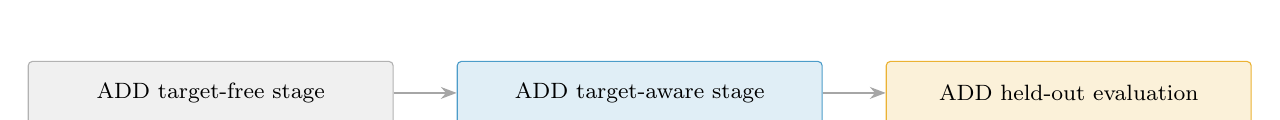
\begin{tikzpicture}[
    node distance=6mm and 8mm,
    box/.style={draw, rounded corners=1.5pt, align=flush center, font=\footnotesize, minimum height=8mm, text width=44mm},
    tfree/.style={box, fill=gray!12, draw=gray!60},
    taware/.style={box, fill=cBlue!12, draw=cBlue!70},
    oot/.style={box, fill=cOrange!15, draw=cOrange!80},
    arrow/.style={-{Stealth[length=2mm]}, gray!70, thick}
]
\node[tfree] (a) {ADD target-free stage};
\node[taware, right=of a] (b) {ADD target-aware stage};
\node[oot, right=of b] (c) {ADD held-out evaluation};
\draw[arrow] (a) -- (b);
\draw[arrow] (b) -- (c);
\end{tikzpicture}
\caption{ADD PIPELINE FIGURE CAPTION. Grey boxes are target-free stages, blue boxes target-aware stages fitted on development data, orange boxes the locked held-out evaluation.}
\label{fig:pipeline}
\end{figure*}

\subsection{Data Preprocessing}
\label{subsec:preprocessing}
ADD: missing-value handling, scaling, categorical encoding, unseen-category handling, and the order of preprocessing and selection.

\subsection{ADD Method Family 1}
\label{subsec:method_family_1}
ADD: definition, implementation, criterion, hyperparameters and retained-feature rule for each method. A method inventory table:

\begin{table*}[htbp]
\centering
\footnotesize
\begin{threeparttable}
\caption{ADD METHOD INVENTORY CAPTION.}
\label{tab:methods}
\begin{tabular}{@{}llL{95mm}l@{}}
\toprule
Method & Family & Role & Labels \\
\midrule
ADD METHOD & ADD FAMILY & ADD one-line description & yes/no \\
ADD METHOD & ADD FAMILY & ADD one-line description & yes/no \\
\bottomrule
\end{tabular}
\end{threeparttable}
\end{table*}

\subsection{ADD Method Family 2}
\label{subsec:method_family_2}
ADD: model or prompt version, inputs, information contract, ranking or selection procedure, caching and reproducibility procedure.

\subsection{ADD Method Family 3}
\label{subsec:method_family_3}
ADD: exact order of operations for each combined pipeline.

\subsection{Development of the Protocol}
\label{subsec:protocol_development}
ADD: protocol versions preceding the final evaluation and which changes moved the results; superseded values are labelled as such.

% ============================================================
% 5. EXPERIMENTAL SETUP
% ============================================================

\section{Experimental Setup}
\label{sec:experimental_setup}

\subsection{Datasets}
\label{subsec:datasets}
ADD: for each dataset, source, observation unit, event definition, time coverage, sample sizes, event rates and feature universe.

\begin{table*}[htbp]
\centering
\footnotesize
\begin{threeparttable}
\caption{ADD DATASET SUMMARY CAPTION.}
\label{tab:datasets}
\begin{tabular}{@{}lccc@{}}
\toprule
 & ADD DATASET 1 & ADD DATASET 2 & ADD DATASET 3 \\
\midrule
Observation unit & ADD & ADD & ADD \\
DEV window & ADD & ADD & ADD \\
DEV $N$ (event rate) & ADD & ADD & ADD \\
OOT window & ADD & ADD & ADD \\
OOT $N$ (event rate) & ADD & ADD & ADD \\
Feature universe & ADD & ADD & ADD \\
\bottomrule
\end{tabular}
\begin{tablenotes}\footnotesize
\item ADD table note if needed.
\end{tablenotes}
\end{threeparttable}
\end{table*}

\subsection{Held-Out DEV/OOT Design}
\label{subsec:dev_oot}
ADD: DEV and OOT construction, cutoff dates, fold construction, what is frozen before the held-out population is opened, and any change to the design made during the study.

\subsection{Predictive Models}
\label{subsec:models}
ADD: full configuration of each backbone, class weighting, solver, seed, iteration count and stopping rule.

\subsection{Feature Budgets}
\label{subsec:feature_budgets}
ADD: how budgets were determined on development data only and when they were frozen.

\subsection{Evaluation Metrics}
\label{subsec:metrics}

\paragraph{ROC-AUC}
ADD: definition and interpretation.

\paragraph{KS}
ADD: definition, formula, direction of improvement.

\paragraph{Brier score}
ADD: definition, formula, direction of improvement.

\paragraph{Capture@10 and Lift@10}
ADD: definition, formula, direction of improvement.

\paragraph{PSI}
ADD: formula, binning and reference construction, frozen-bin procedure.

\paragraph{Nogueira stability}
ADD: formula, universe used in the denominator, aggregation procedure.

\paragraph{Jaccard similarity}
ADD: formula and pairwise fold aggregation.

\subsection{Statistical Inference}
\label{subsec:inference}
ADD: paired test, null hypothesis, confidence-interval procedure, significance level, number of prespecified comparisons and multiple-testing correction.

\subsection{Leakage and Reproducibility Controls}
\label{subsec:leakage_controls}
ADD: leakage controls, seed policy, versioning of data, code and models, and any other safeguards.

% ============================================================
% 6. RESULTS
% ============================================================

\section{Results}
\label{sec:results}

\subsection{Primary OOT Comparison}
\label{subsec:primary_results}
ADD: the prespecified headline comparisons and their inference; separate observations from explanations.

\begin{table*}[htbp]
\centering
\scriptsize
\setlength{\tabcolsep}{3pt}
\begin{threeparttable}
\caption{ADD PRIMARY RESULTS CAPTION.}
\label{tab:primary_results}
\begin{tabular}{@{}lllcll@{}}
\toprule
Case & ADD arm A (AUC) & ADD arm B (AUC) & Reference & $\Delta$AUC [95\% CI] & Holm $p$ \\
\midrule
ADD CASE & ADD & ADD & ADD & ADD & ADD \\
\bottomrule
\end{tabular}
\begin{tablenotes}\scriptsize
\item[a] ADD table note if needed.
\end{tablenotes}
\end{threeparttable}
\end{table*}

% Result figure drawn with pgfplots in the shared "paper" style; replace with \includegraphics if the figure is external.
\begin{figure}[htbp]
\centering
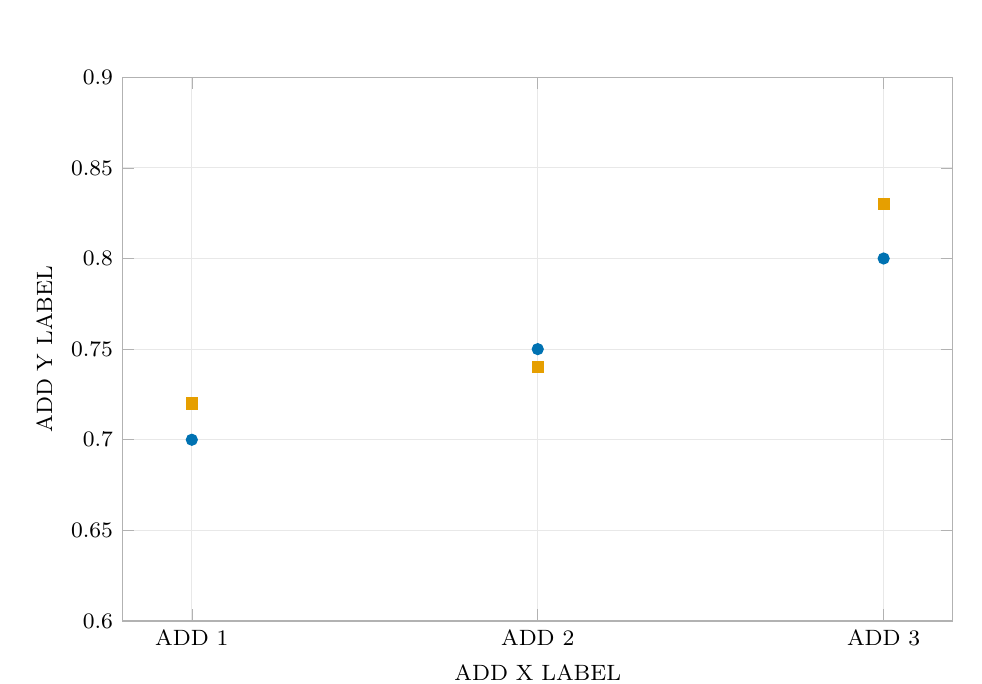
\begin{tikzpicture}
\begin{axis}[
    paper,
    width=\linewidth, height=0.7\linewidth,
    xlabel={ADD X LABEL}, ylabel={ADD Y LABEL},
    ymin=0.6, ymax=0.9,
    xtick={1,2,3}, xticklabels={ADD 1, ADD 2, ADD 3},
    grid=major,
]
\addplot[only marks, mark=*, cBlue] coordinates {(1,0.70) (2,0.75) (3,0.80)};
\addplot[only marks, mark=square*, cOrange] coordinates {(1,0.72) (2,0.74) (3,0.83)};
\end{axis}
\end{tikzpicture}
\caption{ADD FIGURE CAPTION.}
\label{fig:primary}
\end{figure}

\subsection{Secondary Metrics}
\label{subsec:secondary_results}
ADD: secondary metrics without duplicating the primary table.

\subsection{ADD Further Result 1}
\label{subsec:further_result_1}
ADD: numerical results and factual interpretation.

\subsection{ADD Further Result 2}
\label{subsec:further_result_2}
ADD: numerical results and factual interpretation.

\paragraph{Scalability and cost}
ADD: runtime, calls and cost of the proposed stage relative to the baselines, labelled descriptive where measurement conditions differed.

% ============================================================
% 7. DISCUSSION
% ============================================================

\section{Discussion}
\label{sec:discussion}

\subsection{Main Findings}
\label{subsec:main_findings}
ADD: answers to RQ1 to RQn, in the order asked.

\subsection{ADD Trade-off Subsection}
\label{subsec:tradeoffs}
ADD: supported trade-offs between the outcomes measured.

\subsection{Cross-Dataset Behavior}
\label{subsec:cross_dataset}
ADD: which findings reproduce across datasets and models and which are dataset- or model-specific.

\subsection{Limitations}
\label{subsec:limitations}
ADD: limitations of data, models, methods, validation design, inference, reproducibility and generalisability.

% ============================================================
% 8. CONCLUSION
% ============================================================

\section{Conclusion}
\label{sec:conclusion}
ADD: the research question, the strongest supported findings, implications for practice and research, and next steps. Do not introduce new results.

% ============================================================
% END MATTER
% ============================================================

\section*{CRediT authorship contribution statement}
\textbf{ADD AUTHOR 1:} ADD roles. \textbf{ADD AUTHOR 2:} ADD roles.

\section*{Funding}
This research did not receive any specific grant from funding agencies in the public, commercial, or not-for-profit sectors.

\section*{Disclaimer}
ADD: institutional disclaimer if an author is affiliated with a public body, otherwise delete this section.

\section*{Declaration of competing interest}
The authors declare that they have no known competing financial interests or personal relationships that could have appeared to influence the work reported in this paper.

\section*{Data availability}
ADD: repository links or DOIs for datasets, code, cached artefacts and experiment outputs; state the exact reason for anything that cannot be shared.
\begin{itemize}
    \item ADD DATASET: \url{https://ADD-URL}
    \item Code and experiment artefacts: \url{https://ADD-URL}
\end{itemize}

\section*{Declaration of generative AI and AI-assisted technologies in the writing process}
ADD: tool and purpose, followed by the statement that the authors reviewed and edited the content and take full responsibility for it; delete if no such tool was used.

\appendix

% ============================================================
% APPENDICES -- verbatim material such as prompt templates goes in lstlisting blocks
% ============================================================

\section{ADD APPENDIX A TITLE}
\label{app:a}
ADD: one paragraph stating what is reproduced below and where the main text refers to it.

\subsection{ADD listing title}
\label{app:a1}
\begin{lstlisting}
ADD verbatim material (prompt template, configuration, feature list).
\end{lstlisting}

% ============================================================
% REFERENCES -- numbered in order of first appearance; embedded so no BibTeX run is needed
% ============================================================

\begingroup
\footnotesize
\sloppy\hbadness=10000
\begin{thebibliography}{99}

\bibitem{ref1}
ADD: A.~Author, Title, Journal Volume~(Issue) (Year) pages. \url{https://doi.org/ADD}

\bibitem{ref2}
ADD: B.~Author, Title, in: Proceedings, Year, pp.~1--10.

\end{thebibliography}
\endgroup

\end{document}
